\section{Tasas de interés y derivados}

\begin{frame}
% center the title
    \begin{center}
        \textbf{\huge Tasas de interés y derivados}
    \end{center}
\end{frame}
%----------------------------------------------------------------------------------------

\begin{frame}
    \frametitle{Tasa de interés simple}
    Si A le presta un monto \$1 en tiempo $T_1$ a B y B le paga un monto \$1 en tiempo $T_2$ más cierto interés K entre $T_1$ y $T_2$. 
    \begin{figure}[h]
       \centering
       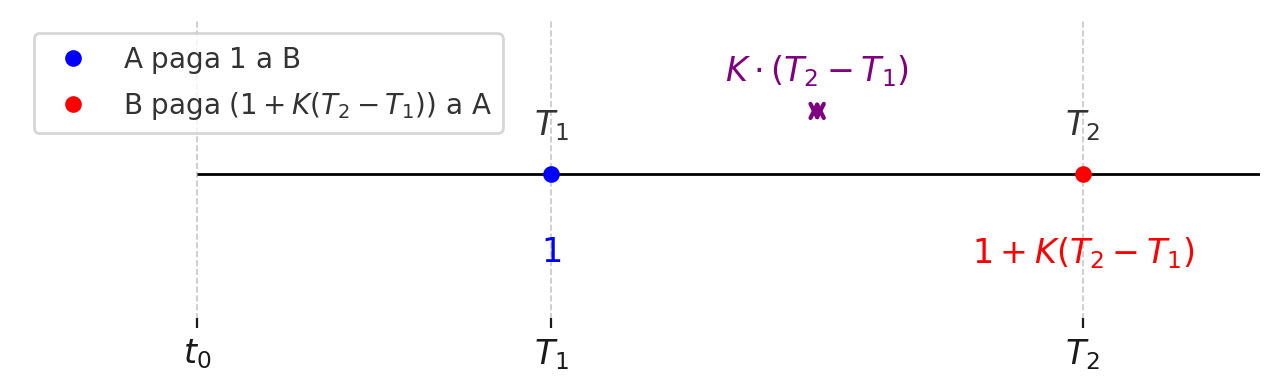
\includegraphics[width=\textwidth]{img/cap1/accrual_simple.png}
       \caption{Tasa simple}
       \label{accrual_simple}
   \end{figure}
\end{frame}

%----------------------------------------------------------------------------------------

\begin{frame}
    \frametitle{Sistemas de Capitalización}
    Un interés de \$100 a una tasa de 10\% anual con capitalización semestral durante 3 años resulta en
    \begin{itemize}
        \item \textbf{Capitalización Simple:} $100 \times (1+\frac{0.1}{2} \times 6) = 130$.
        \item \textbf{Capitalización Compuesta Discreta:} $100 \times (1+0.1/2)^{2 \times 3} = 133.1$.  
        \item \textbf{Capitalización Compuesta Continua:} $100 \times e^{0.1 \times 3} = 134.98$. 
    \end{itemize}

\end{frame}

%----------------------------------------------------------------------------------------

\begin{frame}
    \frametitle{Bonos cupon cero}
    Componentes:
    \begin{itemize}
        \item \textbf{Valor nominal (N):} Monto a pagar al vencimiento.
        \item \textbf{Tasa de interés (r):} Tasa \textit{cero} anual.
        \item \textbf{Tiempo hasta el vencimiento (T):} Tiempo en años hasta el vencimiento.
        \item \textbf{Precio (P):} Precio actual del bono.
    \end{itemize}
    % side by side equations
    \begin{columns}
        \column{0.4\textwidth}
            \begin{equation*}
                P = \frac{N}{(1+r)^T}
            \end{equation*}
        \column{0.4\textwidth}
            \begin{equation*}
                P = N \cdot e^{-rT}
            \end{equation*}
    \end{columns}
\end{frame}

%----------------------------------------------------------------------------------------

\begin{frame}
    \frametitle{Valoración de un bono con cupones}
    Consideremos un bono de principal \$100, madurez en 2 años y tasa cupón 5\% semianual.\\
    Supongamos que las tasas cero a 6 meses, 1 año, 1.5 años y 2 años son 4\%, 4.5\%, 5\% y 5.5\% respectivamente.\\
    \begin{itemize}
        \item \textbf{Flujos de caja:} \$2.5, \$2.5, \$2.5, \$102.5
        \item \textbf{Tasas cero:} 4\%, 4.5\%, 5\%, 5.5\%
        \item \textbf{Precios:} $\$2.5 \cdot e^{-0.04 \cdot 0.5} + \$2.5 \cdot e^{-0.045 \cdot 1} + \$2.5 \cdot e^{-0.05 \cdot 1.5} + \$102.5 \cdot e^{-0.055 \cdot 2}$
        \item \textbf{Precio total:} 98.98
    \end{itemize}
\end{frame}
%----------------------------------------------------------------------------------------

\begin{frame}
    \frametitle{Modelo de tasas de interés}
    \begin{defin}[cuenta de moneda]
        Activo que capitaliza intereses a una tasa de interés r libre de riesgo entre [0, T].\\
        \begin{equation*}
            B(0) = 1 
        \end{equation*}
        \begin{equation*}
            dB(t) = rB(t)dt
        \end{equation*}
        \begin{equation*}
            B(t) = B(0)e^{rt}
        \end{equation*}
        \begin{equation*}
            B(t) = B(0)e^{\int_0^t r(s)ds}
        \end{equation*}
    \end{defin}
\end{frame}

%----------------------------------------------------------------------------------------

\begin{frame}
    \frametitle{Valor inicial de un flujo de caja}
    \begin{defin}[Valor inicial]
        El valor en t=0 de \$1 en t=T es A tal que:
        \begin{equation*}
            A \times B(T) = 1
        \end{equation*}
        \begin{equation*}
            A = \frac{1}{B(T)} = e^{-rT}
        \end{equation*}
        \begin{equation*}
            A = e^{-\int_0^T r(s)ds}
        \end{equation*}
    \end{defin}
\end{frame}
%----------------------------------------------------------------------------------------

\begin{frame}
    \frametitle{Valor presente}
    \begin{defin}[Factor de descuento]
        En $t<T$ el valor presente de \$1 en T es:
        \begin{equation*}
            \frac{1}{B(T)} \times B(t) = \frac{B(t)}{B(T)}
        \end{equation*}
        \begin{equation*}
           D_B(t,T) = \frac{B(t)}{B(T)}
        \end{equation*}
    \end{defin}
\end{frame}

%----------------------------------------------------------------------------------------

\begin{frame}
    \frametitle{Bono cupón cero}
    \begin{defin}[Bono cupón cero]
        Un bono cupón cero P(t,T) es el valor observado en t de un contrato que paga \$1 en T.
        \begin{equation*}
            P(T, T) = 1
        \end{equation*}
        \begin{align*}
            P(t, T) &= D_B(t,T) \\
            &= \frac{B(t)}{B(T)} \\
            \text{si r es estocástica}\\
            &\stackrel{?}{=} D_B(t,T) \\
              &= \mathbb{E}^{\text{???}}\left[\frac{B(t)}{B(T)}\right] \\
        \end{align*}
    \end{defin}
\end{frame}

%----------------------------------------------------------------------------------------

\begin{frame}
    \frametitle{Tasas spot}
    \begin{defin}[Tasa spot simple]
        Es la tasa de interés L vigente entre [S,T] tal que:
        \begin{equation*}
            P(S,T) \times (1+L(S,T) (T-S)) = 1
        \end{equation*}
    \end{defin}
    \begin{defin}[Tasa spot compuesta]
        Es la tasa de interés R vigente entre [S,T] tal que:
        \begin{equation*}
            P(S,T) \times (1+R(S,T))^{(T-S)} = 1
        \end{equation*}
    \end{defin}
\end{frame}
%----------------------------------------------------------------------------------------

\begin{frame}
    \frametitle{Tasas forward}
    Son tasas implícitas por las tasas spot.
    \begin{itemize}
        \item Sean las tasas spot a 1 y 2 años conocidas e iguales a 3 y 4\% respectivamente.
        \item entonces la tasa forward f entre el año 1 y 2 es tal que
        \[e^{0.03} \cdot e^{f(0,1,2)} = e^{0.04 \cdot 2} \therefore f(0,1,2)=0.05 \]
    \end{itemize}
        \begin{figure}[h]
        \centering
        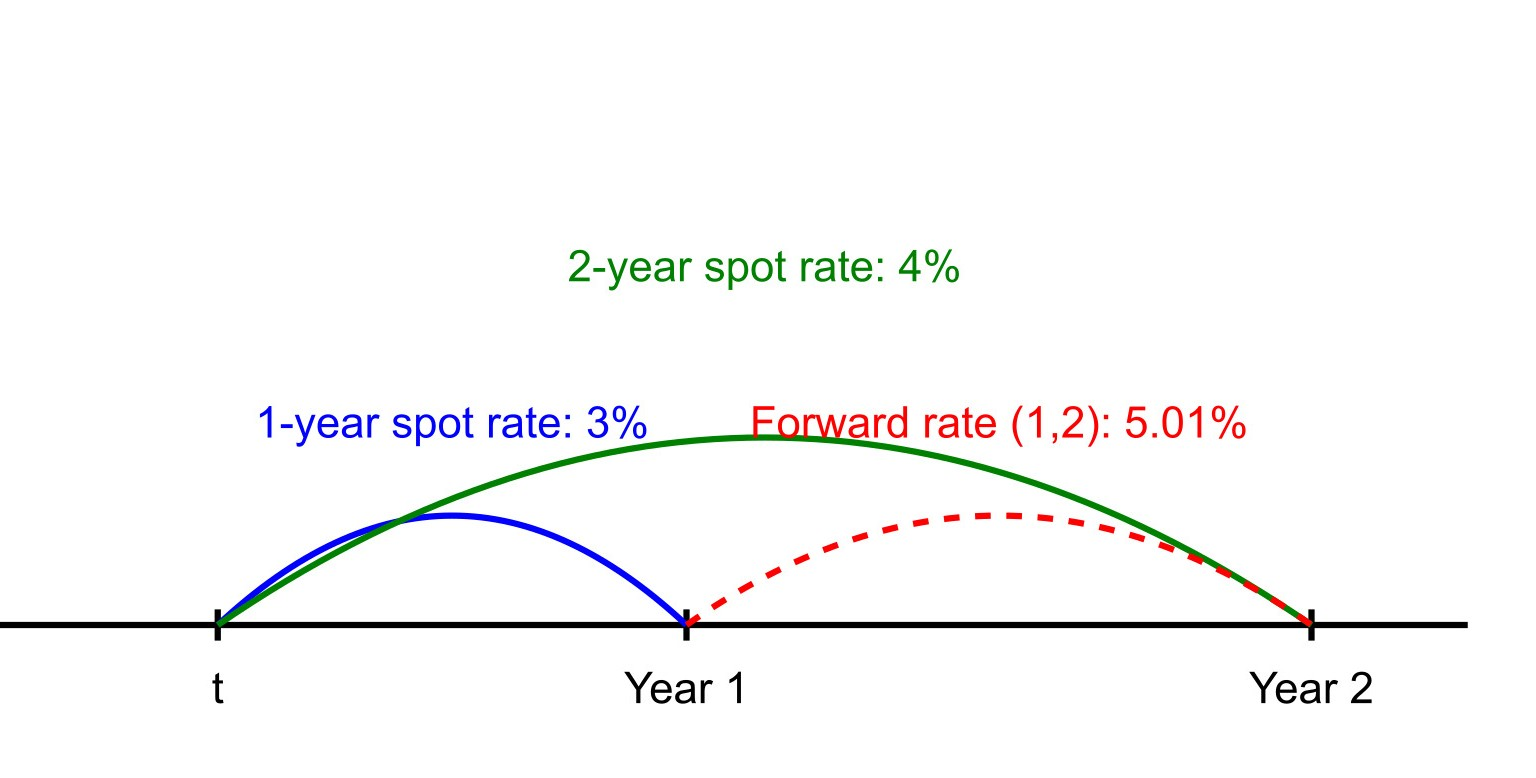
\includegraphics[width=0.8\textwidth]{img/cap1/forward-rates.jpg}
        \caption{Tasas forward}
        \label{forward_rates}
    \end{figure}
\end{frame}

%----------------------------------------------------------------------------------------

\begin{frame}
    \frametitle{Bonos y tasas forward}
    Para capturar un bono que se emitirá en el futuro deberíamos
    \begin{itemize}
        \item Comprar un (1) BCC con madurez $T_2$ y vender alguna cantidad BCC con madurez $T_1$.
        \item El costo de la estrategia es:
        \begin{equation*}
            -1 \cdot P(T_0,T_2) + \frac{P(T_0,T_2)}{P(T_0,T_1)} \cdot P(T_0,T_1) = 0
        \end{equation*}
    \end{itemize}
    \begin{defin}[Bono forward]
        Un bono forward es un contrato que paga \$1 en el tiempo $T_2$ y cuyo precio es
        \begin{equation*}
            P(T_0, T_1, T_2) = \frac{P(T_0,T_2)}{P(T_0,T_1)}
        \end{equation*}
    \end{defin}
\end{frame}

%----------------------------------------------------------------------------------------

\begin{frame}
    \frametitle{Tasas forward}
    \begin{defin}[Tasa forward simple]
        Es la tasa de interés L vigente entre [T,T+$\tau$] tal que:
        \begin{equation*}
            L(t, T, T+\tau) = \frac{1}{\tau} \left( \frac{1}{P(t, T, T+\tau)} - 1\right)
        \end{equation*}
    \end{defin}
    \begin{defin}[Tasa forward continua]
        Es la tasa de interés R vigente entre [T,T+$\tau$] tal que:
        \begin{equation*}
            R(t, T, T+\tau) = \frac{1}{\tau} \cdot \ln\left(\frac{1}{P(t, T, T+\tau)}\right)
        \end{equation*}
    \end{defin}
\end{frame}
%----------------------------------------------------------------------------------------

\begin{frame}
    \frametitle{Tasas forward}
    \begin{notat}
        Denotamos $L_j(t)$ a la tasa forward $L(t, T_j, T_{j+1})$.
    \end{notat}

\end{frame}

%----------------------------------------------------------------------------------------
\begin{frame}
    \begin{center}
        \textbf{\huge Derivados}
    \end{center}
\end{frame}

%----------------------------------------------------------------------------------------

\begin{frame}
    \frametitle{Derivados}
    \begin{defin}[Derivado]
        Un derivado es un contrato cuyo pago es una función de un activo subyacente S en algún momento T.
        \[V(T) = f(S(T))\]
    \end{defin}
\end{frame}
%----------------------------------------------------------------------------------------

\begin{frame}
    \frametitle{Opciones}
    \begin{defin}[Opcion]
        Una opción tiene un desembolso (payoff) que depende del subyacente y un umbral.\\
        \begin{itemize}
            \item Base o strike: umbral para ejercicio.
            \item Fecha de ejercicio: europeas < bermudas < americanas.
            \item Prima: Precio de la opción.
        \end{itemize}
    \end{defin}
\end{frame}

%----------------------------------------------------------------------------------------

\begin{frame}
    \frametitle{Derivados: C50}
    \begin{figure}[h]
       \centering
       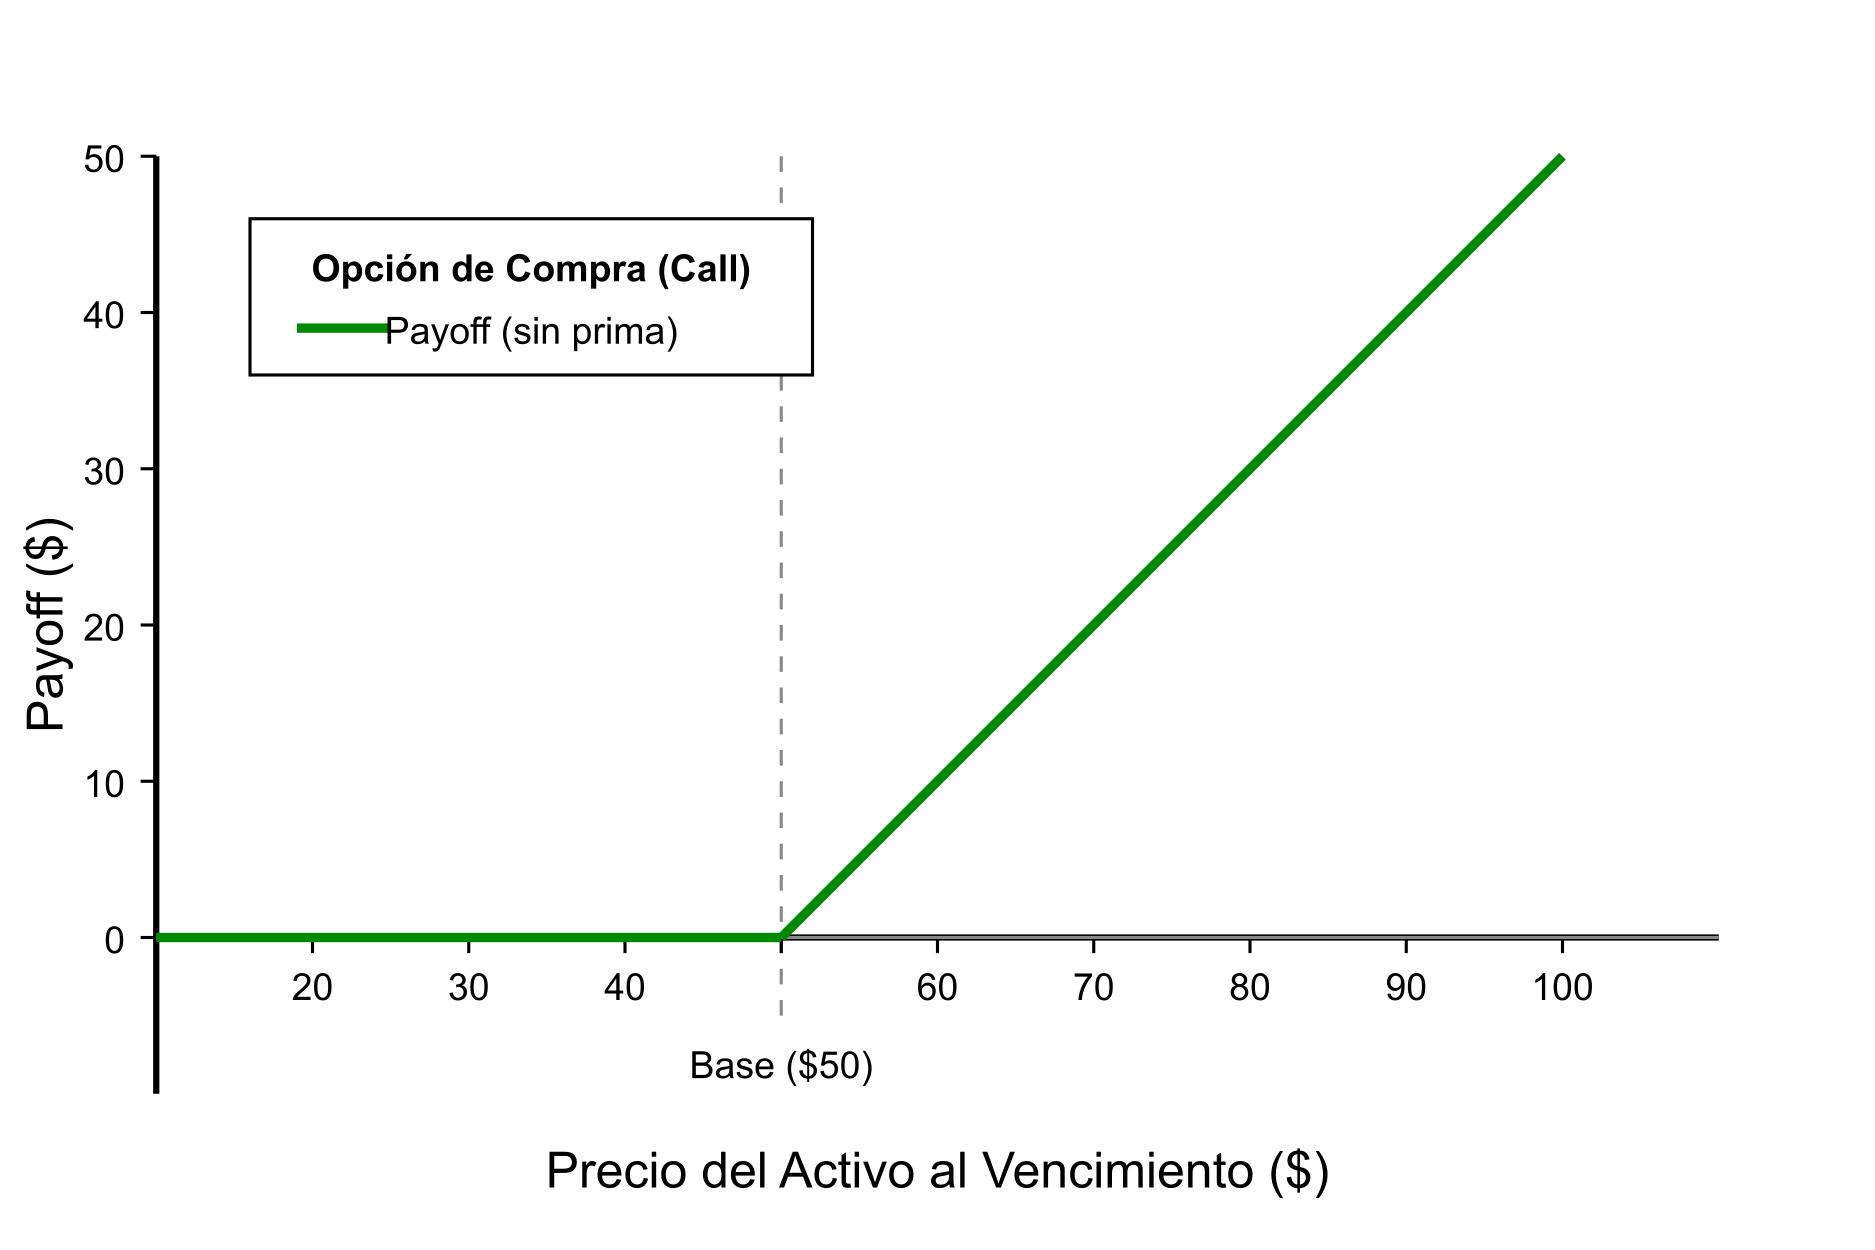
\includegraphics[width=0.8\textwidth]{img/cap1/call50.jpg}
       \caption{Call base 50}
       \label{Call50}
    \end{figure}
\end{frame}

%----------------------------------------------------------------------------------------

\begin{frame}
    \frametitle{FRA}
    \begin{defin}[FRA]
        Un FRA es un contrato que paga la diferencia entre la tasa fija K y otra variable L entre dos fechas $[T_1,T_2]$.
        \begin{itemize}
            \item t=0: fecha de inicio del contrato.
            \item $T_1$: fecha en la que conozco la tasa $L(T_1,T_2)$.
            \item $T_2$: fecha de pago.
        \end{itemize}
        \begin{align*}
            \text{Payoff}_{\text{Short}} &= N (K - L(T_1,T_2)) \cdot (T_2 - T_1), \\
            \text{Payoff}_{\text{Long}} &= N (L(T_1,T_2) - K) \cdot (T_2 - T_1). \\
            \text{K}_\text{FRA} &= L(0, 1, 2) = L_1(0)
        \end{align*}
    \end{defin}
\end{frame}

%----------------------------------------------------------------------------------------

\begin{frame}
    \frametitle{Swap}
    \begin{defin}[Swap]
        \begin{itemize}
            \item Nominal N, Tasa fija K, Tasa variable L
            \item Tiempos de Observación de L: $T_0, T_1, \ldots, T_{n-1}$
            \item Tiempos de pago; $T_1, T_2, \ldots, T_{n}$
            \item Tenor: $T_i - T_{i-1}= \tau_i$
            \item Pago long en cada $T_i$: $N\cdot \tau_i \cdot K$
            \item Pago short en cada $T_i$: $N\cdot \tau_i \cdot L(T_{i-1}, T_i)$
        \end{itemize}
        \begin{align*}
            \text{Payoff}_{\text{Long}} &= N \sum_{i=1}^n \tau_i (L(T_{i-1}, T_i) - K). \\
            \text{K}_\text{Swap} &= \frac{\sum_{j=1}^n P(t, T_{j+1}) (T_{j+1} - T_j) L_j(t)}{\sum_{j=1}^n P(t, T_{j+1}) (T_{j+1} - T_j)}
        \end{align*}
    \end{defin}
\end{frame}

%----------------------------------------------------------------------------------------

\begin{frame}
    \frametitle{Swap: Ejemplo}
    \begin{itemize}
        \item Nominal \$1000, tasa fija 5\%, tasa variable L.
        \item Tiempos de observación de L: 1, 2, 3, 4 años.
        \item Tiempos de pago: 2, 3, 4, 5 años.
        \item Tenor: 1 año.
        \item Pago long en cada $T_i$: \$50
        \item Pago short en cada $T_i$: $L(T_{i-1}, T_i)$
    \end{itemize}
    \begin{align*}
        \text{Payoff}_{\text{Short}} &= \$1000 \cdot \sum_{i=1}^4 (1) (5\% - L(T_{i-1}, T_i)) \\
        \text{Payoff}_{\text{Long}} &= \$1000 \cdot \sum_{i=1}^4 (1) (L(T_{i-1}, T_i) - 5\%)
    \end{align*}
\end{frame}

%----------------------------------------------------------------------------------------

\begin{frame}
    \frametitle{Cap}
    \begin{defin}[Cap]
        Similar al swap, pero el pago es el máximo entre la tasa variable y la tasa fija.
        \begin{align*}
            \text{Payoff}_{\text{Short}} &= N \sum_{i=1}^n \tau_i (K - L(T_{i-1}, T_i))^+ \\
            \text{Payoff}_{\text{Long}} &= N \sum_{i=1}^n \tau_i (L(T_{i-1}, T_i) - K)^+
        \end{align*}
        Compuesto por \textit{caplets}.
    \end{defin}
\end{frame}

%----------------------------------------------------------------------------------------

\begin{frame}
    \frametitle{Floor}
    \begin{defin}[Floor]
        Similar al swap, pero el pago es el mínimo entre la tasa variable y la tasa fija.
        \begin{align*}
            \text{Payoff}_{\text{Short}} &= N \sum_{i=1}^n \tau_i (K - L(T_{i-1}, T_i))^- \\
            \text{Payoff}_{\text{Long}} &= N \sum_{i=1}^n \tau_i (L(T_{i-1}, T_i) - K)^-
        \end{align*}
        Compuesto por \textit{floorlets}.
    \end{defin}
\end{frame}

%----------------------------------------------------------------------------------------

\begin{frame}
    \frametitle{Swaption}
    \begin{defin}[Swaption]
        Un swaption es un contrato que otorga el derecho, pero no la obligación, de entrar en un swap.
        \begin{equation*}
        \text{Payoff}_{T_0} = \max\left(0, N \sum_{i=1}^n \tau_i (L(T_{i-1}, T_i) - K)\right)
        \end{equation*}
    \end{defin}
\end{frame}

